% !Rnw weave = knitr
\documentclass[12pt]{article}\usepackage[]{graphicx}\usepackage[]{color}
%% maxwidth is the original width if it is less than linewidth
%% otherwise use linewidth (to make sure the graphics do not exceed the margin)
\makeatletter
\def\maxwidth{ %
  \ifdim\Gin@nat@width>\linewidth
    \linewidth
  \else
    \Gin@nat@width
  \fi
}
\makeatother

\definecolor{fgcolor}{rgb}{0.345, 0.345, 0.345}
\newcommand{\hlnum}[1]{\textcolor[rgb]{0.686,0.059,0.569}{#1}}%
\newcommand{\hlstr}[1]{\textcolor[rgb]{0.192,0.494,0.8}{#1}}%
\newcommand{\hlcom}[1]{\textcolor[rgb]{0.678,0.584,0.686}{\textit{#1}}}%
\newcommand{\hlopt}[1]{\textcolor[rgb]{0,0,0}{#1}}%
\newcommand{\hlstd}[1]{\textcolor[rgb]{0.345,0.345,0.345}{#1}}%
\newcommand{\hlkwa}[1]{\textcolor[rgb]{0.161,0.373,0.58}{\textbf{#1}}}%
\newcommand{\hlkwb}[1]{\textcolor[rgb]{0.69,0.353,0.396}{#1}}%
\newcommand{\hlkwc}[1]{\textcolor[rgb]{0.333,0.667,0.333}{#1}}%
\newcommand{\hlkwd}[1]{\textcolor[rgb]{0.737,0.353,0.396}{\textbf{#1}}}%
\let\hlipl\hlkwb

\usepackage{framed}
\makeatletter
\newenvironment{kframe}{%
 \def\at@end@of@kframe{}%
 \ifinner\ifhmode%
  \def\at@end@of@kframe{\end{minipage}}%
  \begin{minipage}{\columnwidth}%
 \fi\fi%
 \def\FrameCommand##1{\hskip\@totalleftmargin \hskip-\fboxsep
 \colorbox{shadecolor}{##1}\hskip-\fboxsep
     % There is no \\@totalrightmargin, so:
     \hskip-\linewidth \hskip-\@totalleftmargin \hskip\columnwidth}%
 \MakeFramed {\advance\hsize-\width
   \@totalleftmargin\z@ \linewidth\hsize
   \@setminipage}}%
 {\par\unskip\endMakeFramed%
 \at@end@of@kframe}
\makeatother

\definecolor{shadecolor}{rgb}{.97, .97, .97}
\definecolor{messagecolor}{rgb}{0, 0, 0}
\definecolor{warningcolor}{rgb}{1, 0, 1}
\definecolor{errorcolor}{rgb}{1, 0, 0}
\newenvironment{knitrout}{}{} % an empty environment to be redefined in TeX

\usepackage{alltt}
\usepackage[backend=biber, sorting=nyt, maxcitenames=2, doi=false,url=false, style=apa]{biblatex} %add annotation=true and style=reading to print the annotations in the bibliography
\usepackage[american]{babel}
%\usepackage{newtxtext,newtxmath}
\usepackage{csquotes}
\bibliography{/Users/Owner/Documents/Tex/all,/Users/Owner/Documents/Thesis/thesis_ref}
\DeclareLanguageMapping{american}{american-apa}
\usepackage[compact]{titlesec}
\usepackage{csquotes}
\usepackage{amsmath}
%\usepackage[hyphens]{url}
\usepackage[margin=1in]{geometry}
\usepackage{mathtools}
\setlength{\parskip}{.6em}
\usepackage{setspace}
\usepackage{multicol}
\usepackage{longtable}
\usepackage{makecell}
\renewcommand\theadalign{bc}
\renewcommand\theadfont{\bfseries}
\renewcommand\theadgape{\Gape[4pt]}
\renewcommand\cellgape{\Gape[4pt]}
\renewcommand{\tablename}{Table}
%\usepackage{sectsty}
%\allsectionsfont{\singlespacing}
%\usepackage{indentfirst} %This indents the pfaragraph following a heading 
\setlength{\parindent}{0em}
\usepackage{breqn}
\usepackage{graphicx}
\usepackage{pdfpages}
\usepackage{subcaption}
\usepackage[figuresleft]{rotating}
\graphicspath{{C:/Users/Owner/documents/github/eysterthesis/manuscript/}} %make sure to include the slash after the colon at at the end 
%Make sure Bibliography --> is set as biblatex 
%Then run tools-->bibliography, then compile 
\usepackage{authblk}
\title{Invader success and changing climate: Comparisons in the native and introduced range of seven plant species}
\author[1]{Harold N. Eyster}
\author[2]{Elizabeth Wolkovich}
\affil[1]{Institute for Resources, Environment, and Sustainability, University of British Columbia}
\affil[2]{Department of Forest and Conservation Science, University of British Columbia}
\date{}                     %% if you don't need date to appear
\setcounter{Maxaffil}{0}
\renewcommand\Affilfont{\itshape\small}






\IfFileExists{upquote.sty}{\usepackage{upquote}}{}
\begin{document}
\maketitle
%	\fbox{\includegraphics[width=1 \textwidth,trim=0cm 0cm 0cm 0cm, clip=true]{comps_overview}}

\begin{spacing}{1} %1.9
	\begin{abstract}
		Invasive species can have transformative impacts on native ecosystems. Yet the strategies that plants employ to invade novel ecosystems remain poorly understood.  Two factors that may enable plants to successfully invade a range of environments are local adaptation and plasticity. Phenological traits (recurring life-cycle events, such as flowering) are sensitive to climate and directly related to success in a given environment. This research experimentally tests the relative importance of phenological local adaptation and plasticity in driving invasion success. Seeds from seven herbaceous plant species were collected from multiple populations in their native (European) and invasive (American) ranges. The seeds were subjected to two stratification treatments (to simulate different winter lengths) and then planted in growth chambers at a range of  four temperatures. Phenological traits were measured for each seed (germination rate, germination timing, and growth rate). Using these measurments to  fit Bayesian hierachical mixed effects models, we found consistent and significant evidence that the in phenological adaptation  No general patterns were found across species or population origin (i.e., American vs. European) in the relative plasticity of phenological traits, suggesting that adaptive plasticity may be important for some species but not others. However, the invasive American populations consistently showed evidence of local adaptation to the environment. My study demonstrates that the capacity of invasive species to adapt to different winter lengths (i.e., stratification) and temperatures will likely allow them to adapt to the novel seasons and temperatures associated with global climate change.  
	\end{abstract}
\end{spacing}		
	\section{Introduction}
	As invasive species colonize new environments they have important, often transformative, effects on ecosystems \parencite{Mack2000,Levine2003}.  Exotic plant invasions have large impacts on biodiversity \parencite{Bellard2016,Clavero2005,Walker1997}, ecosystem function, services,and resilience \parencite{Daehler1999,Daehler1994,Ehrenfeld2003,Wilcove1998,Pejchar2009,Pimentel2005,Pysek2010,OTA1993}.  And invasions may only be increasing: globalization is making it easier for plants to disperse beyond their native ranges \parencite{Helmus2014,McKinney1999,Pysek2002,Vitousek1996,Wittenberg2001}. However, mere dispersal to a new environment is insufficient to entail invasiveness. Upon encountering a new environment, an invasive species must thrive, often by either filling vacant niches \parencite{Elton1958} or outperforming native plants in high-resource and variable environments \parencite{Davis2001,Daehler2003}. The availability of these invasible environments are likely to increase when ecosystems are altered \parencite{Tilman2001}. Anthropogenic greenhouse gas pollution and  habitat modification will likely disrupt communities and provide vacant niches and altered resource availability; such changes could provide major opportunities for invasive species to outperform native plants \parencite{Blois2013}. In particular, greenhouse gases are altering temperature and irradiance, which is shifting temporal niche space and disrupting communities \parencite{Inouye2008,Harte2015}. This changing environment could select for species that can take advantage of the newly created temporal niches and resources through shifts in the timing of flowering and fruiting, etc. \parencite{Franks2007}. Two contrasting mechanisms have been posited to give some plants the capacity to exploit invasible environments: 1) rapid evolution and 2) plastic or generalist traits.  This paper tests the importance of these two mechanisms. 

	%To invade new The first factor for determining invasion potential is dispersal. To become invasive, a species first needs a dispersal mechanism to establish in a non-native habitat \parencite{Mark2001,Westphal2008}. Humans have played an important role in facilitating recent plant dispersals \parencite{McKinney1999,Pysek2002,Vitousek1996}, and with increased globalization the spread of species outside their respective native ranges will only increase \parencite{Helmus2014}. Once a species is introduced to a novel region, however, it must also be able to successfully disperse beyond the initial introduction location to be considered fully invasive. Thus species with greater dispersal ability may be more successful invaders.  Nonetheless, any intrinsic biological dispersal advantage can be wholly dominated by intentional introduction, e.g., for agricultural or ornamental purposes, or by accidental human-facilitated mechanisms, such as the transportation of invasive species within contaminated mulch or gravel \parencite{Wittenberg2001}. 	
	%Managing this onrush of invasive species requires understanding the mechanisms that give some plants the capacity to exploit invasible environments \parencite{Hulme2013}
	
	A large body of literature suggests that rapid adaptive evolution is a key determinant of success in invading of new environments \parencite{Sakai2001,Reznick2001, Lambrinos2004,Williamson1997,Thompson1998, Cox2004, Prentis2008,Colautti2015,Lee2002invasion, Fenollosa2019,Clements2011}.  Rapid evolution can enable nonindigenous species to adapt to vacant niches and take advantage of variable and high-resource environments, for example by evolving greater competative ability  when released from natural enemies \parencite{Blossey1995,Bossdorf2005} or by evolving adaptive plasticity \parencite{Richards2006}. Many genetic characteristics have been identified to enable invasion, including additive genetic variation, epistasis, hybridization, genomic rearrangements, etc. \parencite[Reviewed in][]{Lee2002invasion}, while genetic drift and bottlenecks likely stifle invasion capacity \parencite{Bock2015}. 
	
	There are many clear examples of rapid evolution abetting plant invasions. For instance, genetic studies of two herbaceous goldenrods that invaded Europe from North America, \textit{Solidago altissima} and \textit{S. gigantea} (Asteraceae), showed post-introduction genetic changes in flowering time in response to temperature, due to selection on source-population genetic variation and development of new mutations \parencite{Weber1998}. Similarly, the invasive \textit{Centaurea solstitialis} (Asteraceae) in California evolved larger size from standing variation in the founding population \parencite{Barker2017}. Also in California, a similar study found that genetic adaptation was driving adaptive phenotypic variation in flowering time of high-altitude and desert populations of \textit{Capsella bursa-pastoris} \parencite{Linde2001}. Invasion may even produce evolution sufficient to establish reproductive isolation and trigger speciation, in as few as 13 generations \parencite{Hendry2000}. If rapid evolution is so central to invader success, then managers should treat invasives not as static, homogeneous species, but as constantly adapting populations \parencite{Lee2002invasion}. 
	
	Yet, dispute the support for the importance of rapid evolution, a competing body of literature suggests that invaders need not evolve. Instead,  plasticity and generalist adaptations to human-dominated environments (i.e., weediness) within the source population may give invaders sufficient advantages, obviating the necessity of rapid evolution \parencite{Richards2006,Schwartz1994}. Species that are weedy and invasive in their native range are likely to be invasive in novel environments: a study of 274 plant species native to North and South America but naturalized in France showed that the best determinant of invasiveness was weediness in the home range \parencite{Maillet2000}.
	
	One reason why the importance of rapid evolution remains contested is because few experimental designs allow unambiguous discrimination between the two claims. Neither observational datasets (e.g., \parencite{Wolkovich2013} nor experimental common gardens \parencite{Conner2004,Vitasse2009} are sufficient to identify the importance of rapid evolution.   And while genetic studies can identify the existence of rapid evolution, they do not demonstrate the dominance of this invasion technique. Instead, reciprocal common garden or  growth chamber experiments with origin and invader populations are necessary to disentangle these competing theories. One such reciprocal common garden experiment of two invasive maple species (\textit{Acer}, Sapindaceae) demonstrated that rapid evolution was important for one species, but not the other \parencite{Lamarque2015}. Additional reciprocal common garden experiments have examined single species \parencite[e.g.,][]{Williams2008}. Due to the limited number of species tested with these methods, the overall necessity of rapid evolution for invaders remains hidden.
	
	Seeking this more general appraisal of the importance of rapid evolution for invaders, this paper reports on a growth chamber experiment of the native and introduced ranges of seven highly invasive herbaceous plant species. We test the degree to which rapid evolution has occurred since the species colonized North America from Europe.  Our growth chamber experiment enabled us to test the degree to which phenologies in native and invasive populations differ in their response to climate.   Specifically, we measured how germination rate, time to germination, and growth rate of invasive (American) and native (European) conspecific populations responded to an array of temperature and stratification treatments.
	
	This study manipulates two key climate elements: temperature and stratification length. Temperature and stratification length act as important phenological cues for plants \parencite{Finch2006}. In temperate ecosystems, a cold stratification simulates winter. A minimum period of winter must often pass before seeds can germinate. This ensures that seeds will not germinate during a mid-winter warm period, but instead wait until a spring warm period when winter has fully passed. Thus, exposing dormant seeds to a variety of stratification lengths elucidates how they respond to different winter lengths. Once the necessary stratification length has been achieved, temperature can cue that it is the appropriate time for a seed or plant to break dormancy. Temperature also plays an important role in controlling plant growth rate \parencite{Egli1980,Guilioni2003}.
	
	Temperature and stratification length are appropriate variables for studying invasive vs. native plant phenology. These abiotic factors effectively trigger phenology, and can simulate diverse geographic environments. Additionally, temperature and stratification reflect different aspects of the seasonal environment: stratification length is associated with winter, while warmer temperatures are associated with the growing season. Including drivers such as stratification from the non-growing season is important, given that winter climate may change independently from summer climate, and that winter climate varies more spatially \parencite{Bonan2003}. Thus, a range of temperature and stratification treatments will simulate the driving features of the diverse environments in which invasive species thrive. 
	
	 If rapid evolution is of generalizable importance to invasive plants, we expect to find that seeds from the invading populations (North America) will respond very differently to temperature and stratification treatments than the indigenous populations (Europe) for all or nearly all species. Isolating the importance of rapid evolution in such a complex multispecies, multi-population design would be intractable with classic frequentest modeling  techniques. Fortunately, advances in Bayesian and hierarchical modeling have provided methods that enable interpretation of our data \parencite{Carpenter2017}.  These methods will provide a robust test of the claim that rapid evolution drives invader success.
	 
	\section{Methods}
	\subsection{Study species}
	%can probably cut: 
	There is no consensus on what terminology to employ in classifying invasive species \parencite{Colautti2004}. The most common terms include `exotic,' `introduced,' `naturalized,' `nonindigenous,' `established,' `alien,' `noxious,' `weedy,' and `invasive.' These terms can be grouped into those that describe the provenance of the species (e.g., exotic, introduced, alien, non-indigenous), those that describe its ability to grow and compete in the new ecosystem (e.g., naturalized, established), and those that describe its impact on the receiving ecosystem (e.g., noxious, weedy, harmful). The International Union for the Conservation of Nature (IUCN) describes invasive species as: ``organisms introduced by man [sic] into places out of their natural range of distribution, where they become established and disperse, generating a negative impact" \parencite{IUCN2008is}. However, this definition contains three subjective elements: what timepoint of a species' range is `natural,' whether humans are a natural part of nature, and what is defined as a negative impact \parencite{Munro2019}. To both acknowledge and allay some of these subjective elements, this paper will follow Richardson et al.'s \parencite{Richardson2000,Richardson2011} definition of invasive species. Invasive species are thus those that (1) are introduced across a previously unpenetrated barrier, (2) successfully reproduce in the place of introduction to create a stable local population, and finally (3) spread to produce fit offspring a substantial distance from the place of introduction.
	
	Guided by this definition, seeds were collected from eight herbaceous species that originated in Europe but have recently been introduced to the US, where they have spread and produced significant populations:\textit{ Alliaria petiolata, Capsella bursa-pastoris, Chelidonium majus, Dactylis glomerata, Plantago major, Plantago lanceolata, Rumex crispus, and Taraxacum officinale}.\textit{A. petiolata} exhibited very low germination rates, and so was removed from the analysis.  All of these species have proven prodigious invaders in the US, with many impacting crop production and transforming ecosystems \parencite[e.g.,][]{Froese2003,Wolfe2008}. The study species (see Table \ref{tab:seeds}) were selected for their occurrence in Europe and for their superior invasive capacity in their introduced range \parencite{Uva1997}, since the most unambiguous response may be obtained by examining the most extreme invasive species, and may also be most useful for informing management. 
	\begin{center}
		\begin{table}
			\centering
			\caption {Total number of seed-producing individuals and populations from which seeds were collected. Species are coded as the first three letters of the genus plus the first three letters of the species epithet.} \label{tab:seeds}  
			\begin{tabular}{|c|c|c|c|}
				\hline 
				\makecell{\textbf{US} \\ \textbf{populations}} & \makecell{\textbf{US} \\  \textbf{individuals}} & \makecell{\textbf{European} \\ \textbf{populations}} & \makecell{\textbf{European} \\ \textbf{individuals}} \\
				\hline
				3&	21&	13&	63\\
				\hline
			\end{tabular}
		\end{table}
	\end{center}
	\subsubsection{Study species details}
	\textit{Capsella bursa-pastoris} (CAPBUR;Shepard’s Purse) is an annual or biennial herbaceous plant in the Brassicaceae family. It grows 10 to 80 cm tall, typically blooming in late spring \parencite{Defelice2001}. It originated in Europe, and was introduced to the New World as a medicinal herb---it is now found across Canada, the US, and Mexico \parencite{Westrich1989}.
	
	\textit{Chelidonium majus} (CHEMAJ; Greater Celandine) is an herbaceous biennial member of Papaveraceae. It is native to Eurasia and North Africa and was introduced to the US by the 1670s as a medicinal. It is now found across the Eastern US and Canada and portions of the west \parencite{Holm1979}. 
	
	\textit{Dactylis glomerata} (DACGLO; Orchard Grass) is a cool-season, perennial grass (Poaceae). Plants grow up to 120 cm tall and have roots up to 60 cm long \parencite{Moser1996}. This plant originated in central and western Europe, and was intentionally introduced into the US in the 1750s \parencite{Bush2012} as a forage grass for pasture and hay \parencite{Ogle2011}.  
	
	\textit{Plantago lanceolata} (PLALAN; Narrow-leaved Plantain) is a perennial member of  Plantaginaceae. It has narrow, ribbed leaves and grows to 1m tall. It is native to Eurasia, and has successfully colonized the world’s mid-latitudes \parencite{Holm1977}.
	
	\textit{Plantago major} (PLAMAJ; Broad-leaved Plantain) is a perennial member of Plantaginaceae. It has broad, smooth leaves, and grows to 15cm tall. Native to Europe, it was introduced into North America for its medicinal uses \parencite{Knobloch1996,Samuelsen2000}.
	
	\textit{Rumex crispus} (RUMCRI; Curly Dock) is a perennial herbaceous plant in Polygonaceae, and grows to 160 cm. It is native to Europe, Asia, and Africa, and was introduced for its medicinal uses into North America where it now found across much of the continent \parencite{USDA2010}. 
	
	\textit{Taraxacum officinale} (TAROFF; Dandelion) is a perennial herbaceous plant in the Asteraceae family, and grows to 60 cm. It is native to Eurasia, but is now found in all 50 US states, much of Canada, and Mexico \parencite{USDA1971}.
	
	\subsection{Seed collection}
	Seeds were collected from native populations in Europe and invasive populations in North America from June 15th to September 5th 2015. Mature seeds were collected from individual plants and placed into paper coin envelopes. The following data were recorded for each individual plant: species, date, name of site, notes on human disturbance at site, abundance of the species at the site, aspect, elevation, GPS coordinates, height of the individual, spread of the individual, photo of the site, photo of at least one individual/site, and soil type. The seeds were then stored at standard room temperature until early September 2015, at which time all of the seeds were cleaned and returned to envelopes. 
	\paragraph{European (native) seed collection} 
	Seeds were collected in Europe from early-June to mid-July 2015 from 13 sites across 9 European countries: France, The Netherlands, Germany, Denmark, Norway, Austria, Slovenia, Liechtenstein, and Switzerland (see Figure \ref{fig:sites}). Seeds from European populations were collected from elevations ranging from 0-1202 m above sea level (see Figure 2). Plant seeds were imported into the United States with a USDA small seedlot permit, which required that no more than 50 seeds be collected per envelope. Thus, typically 50 seeds/individual were collected. See Table \ref{tab:seeds} for details about the number of populations and individuals sampled. 
   \paragraph{North American (nonnative) seed collection} Seeds were collected in North America from June through early September from three sites in Massachusetts, United States:  Harvard Forest (N 42.53096, W -72.19085), Arnold Arboretum at Harvard University, Boston (N 42.30196, W -71.12448), and Walden Pond, Concord (N 42.43927, W -71.3441) (see Figure \ref{fig:sites}). These sites range in elevation from 20 meters to 300 meters. 
	
	\paragraph{Climate}
	To examine how climate varied between populations and continents, the mean March, April, and May temperatures (~ 1 km$^2$ resolution) for 1970-2000 for each population location were downloaded from WorldClim Version 2 \parencite{Fick2017}  and plotted (see Figure \ref{fig:sites}). 
	
	
	\begin{figure}
		\centering
		\fbox{\includegraphics[width=1 \textwidth,trim=0cm 0cm 0cm 0cm, angle=0, scale=.9, origin=c,clip=false]{sampling_sites}}
		%x x x lower right 
		\caption{Map of collection sites of (A) invasive populations in New England and (B) native populations in Europe and (C) average Spring temperatures at each site}
		\label{fig:sites}
	\end{figure}

%	\begin{figure}
%		\centering
%		\fbox{\includegraphics[width=1 \textwidth,trim=0cm 0cm 0cm 0cm, angle=0, scale=.7, origin=c,clip=false]{Elevation-chart}}
		%x x x lower right 
%		\caption{Count of European individuals collected at different altitudes. }
%		\label{fig:elev}
%	\end{figure}
	\subsection{Experimental Design}
	To test germination rates in response to climate, seeds were exposed to eight treatments representing varying climates. Seeds were first subjected to two stratification treatments (varying length of stratification), and then each stratification group was divided between four germination treatments (varying temperature). All treatments were carried out in growth chambers. For each treatment, ten representatives of each species (with seven invasive species this leads to 140 seeds per treatment) and an additional five representatives of each local population of \textit{Plantago lanceolata} (the most heavily sampled species, which had a total of 13 populations, this leads to an additional 65 seeds per treatment) were planted in soil. Germination date, the percentage of seeds germinating, and aboveground linear height were recorded.  A total of 205 seeds were planted per treatment.  Local population representatives were drawn from the greatest variety of individuals (seed families), and the individual make-up was consistent across treatments. 
	
	\subsection{Stratification}
	Stratification is crucial for many species to break organic dormancy and germinate successfully \parencite{Baskin1998,Popay1970,Wulff1994} and how long winter cold lasts (in the form of snow) has been shown to be a key in driving ecological community shifts (Harte et al. 2015). Additionally, with changing climate, winter length is a key niche variable. Studies show stratification of these species vary from 16 days \parencite{Popay1970} to 120 days \parencite{Meekins1999}. This experiment thus used intermediate lengths of 30 and 60 days, respectively, for our two stratification treatments. Seeds in the longer stratification treatment were stratified in late September 2015, while the other seeds in the shorter treatment continued to be stored in paper envelopes at room temperature until they were in turn stratified in late October 2015. Stratification conditions were kept constant across treatments:  4$^\circ$C, 70\% humidity, 380 ppm of $CO_2$ (the standard, see e.g., \textcite{Meekins1999,Popay1970}), seeds were stratified on moistened Whatman 1 qualitative filter paper in Greiner bio-one 94x16 petri dishes (with vents, greiner light version, sterile) in the dark \parencite{Baskin1998,Popay1970}.  Water was added to petri dishes every 30 days. Seeds were stratified in a single Biochambers TPC-19 Reach-In Growth Chamber. 
	
	\subsection{Germination }
	On November 23, 2015, seeds from both stratification treatments were transferred from their petri dishes into individual pots with soil (see Experimental Design, above), which were placed into four different growth chambers (three Biochambers TPC-19 Reach-In Growth Chambers and one Biochambers LTCB-19 Reach-in Growth Chamber) and subjected to four different germination treatments. Temperature varied across treatments---all other measured variables were kept constant, and treatments were rotated through growth chambers to control for the unmeasured chamber effects. Some of the seeds had germinated during stratification. These were noted and discarded.
	
	\paragraph{Germination Temperature:} Popay and Roberts (1970) show that Capsella bursa-pastoris germinates best at 25-30$^\circ$C, and 20-30$^\circ$C seems to be the standard temperatures for optimal weed germination \parencite{Hartmann2010,Steinbauer1957,Wulff1994}. This experiment used a slightly-broadened spectrum to achieve a greater variance in germination success, using temperatures between 18 and 32$^\circ$C. 
	
	\paragraph{Thermoperiocity:} About 80\% of weeds studied in \textcite{Steinbauer1957} and about 75\% of cultivated seeds germinate better with thermoperiocity (i.e., daily fluctuations in temperature)\parencite{Toole1963,ISTA1954}. Thus thermoperiocity of 10 degrees C was used \parencite[see e.g.,][]{Steinbauer1957}, translating to treatment temperatures of: 18/8$^\circ$C, 22.67/12.67$^\circ$C, 27.33/17.33$^\circ$C, and 32/22$^\circ$C. All treatments were subjected to 8 hours at the high temperature and the remaining 16 hours at the low temperature \parencite{Baskin1998,Roberts1981,Popay1970,Probert2000}.
	

	\paragraph{Light type:} Germination rates typically increase when seeds are exposed to light \parencite[e.g.,][]{Baskin1998,Pons2000,Popay1970}. Different studies suggest that the ratio of far to far-red light (R:FR) matters either a lot or not at all for successful germination \parencite[e.g.,][]{Popay1970,Pons2000,Wulff1994}. But, generally, exposure to a high R:FR ratio, increases germination rates. Thus, our experiment used T5HO fluorescent lights \parencite{Toole1963}, which have a high R:FR ratio. 
	
	\paragraph{Period/luminance of light:} Some species have sufficient Pfr (the active form of phytochrome pigment, often necessary to induce germination) and so do not need any light to break dormancy, others just need a pulse of red light to break dormancy (the red light converts the inactive phytochrome into Pfr) \parencite{Casal998}.  Other species, including \textit{Plantago major}, take much longer to build up the requisite Pfr, and so have much higher germination success when exposed to longer periods of light (with nearly 100\% germination after 48 hours of exposure for \textit{P. major}) \parencite{Pons1991}. Finally, some species have a high irradiance response (HIR), expressing poor germination when exposed to high luminance light or prolonged light \parencite{Roberts1987}. Beyond interspecific variation, there is also intraspecific variation in the relationship between dormancy and light \parencite{Probert1986}. Across all populations, germination rate seems to be log-normally related to photon dosage \parencite{Ellis1986}. Light may begin inhibiting germination for HIR species at about 0.1 mol/m2/day – 1 mol/m2/day \parencite{Baskin1998,Ellis1986}, while other species peak above 10 mol/m2/day \parencite{Ellis1986}. The differing levels of light necessary to break dormancy means that any chosen light regime will be better for some species and worse for others. 
	
	The goal of these experiments is to create germination rates that are sufficient to observe variation in responses to treatments. Thus, we chose an intermediate light exposure at which all of the species should germinate at substantial levels, but which may not be ideal for any species. In selecting how much light to use, this experiment erred on the side of too much light rather than not enough, since at least one of our species is known to need large amounts of light (\textit{Plantago major}---\textcite{Pons1991}), and none are known to exhibit HIR (although a \textit{D. glomerata} subspecies in southern Europe does exhibit HIR \parencite[Probert et al., 1986], but this subspecies is not thought to have been collected for this study). Thus this experiment used a length of eight hours at a luminance of 75 micromol/m2/second to yield a daily photon dosage of 2.16 mol/m2. \textcite{Baskin1998} recommend that the light period coincide with the high-temperature period. Thus, this experiment exposed the seeds to eight hours of fluorescent light during the high-temperature thermoperiod. 
	
	\paragraph{Substrte and planting depth:} \textcite{Popay1970} show that \textit{C. bursa-pastoris} seeds germinated about equally on filter paper as on top of soil, but showed much decreased germination when inserted into soil. The effects of planting substrate and depth have not been studied in most of the study species. However, a study on a species related to \textit{D. glomerata} suggests that \textit{D. glomerata} may germinate better in soil \parencite{Andrews1974}. Additionally, a difference in depth of just a couple millimeters can result in extreme differences in light availability \parencite{Tester1987}. Thus each seed was placed on top of Fafard Growing Mix (a mixture of fine peat moss, fine perlite, and vermiculite) soil, with each seed in its own individual tray cell.
	
	\paragraph{Water:} Every two days, seeds were watered until all of the soil had become wet \parencite{Steinbauer1957}; but not so much that a film of water covered the seeds \parencite{AOSA1960}.
	
	\paragraph{Germination monitoring:} Seeds were checked during the light period for germination every two days. Germination success was defined as the growth of shoot or radical through the seed coat \parencite{Baskin1998,Popay1970}. Germination date for each seed was recorded. Data collection sheets only contained the tray location of the seeds, (not population or individual), so collection of germination data was blind to population.  Germination trials typically last two weeks, with most seeds germinating within 10 days \parencite{Baskin1998}. However, after 10 days, new germinations were still being observed so the observation time was extended \parencite{Wulff1994}.
	
	\subsection{Growth}
 	Most of the study species are perennials or biennials. As such, they do not flower in the first year. Instead of floral state, the seeds in the cells growing on soil were analyzed post-germination for height. Aboveground linear height of each seedling was measured five times: on December 7, 2015, December 15, 2015, December 21, 2015, January 4, 2016, and January 29, 2016. On January 1, 2016, the plants were moved from the growth chambers to a greenhouse subject to the following conditions: natural photoperiod (approximately 10 hours of light/day), 20 to 25$^\circ$C, and 65\% humidity.  
 	

	\subsection{Statistical analysis}
	Height was linearly associated with day, so growth rate (in cm/day) was defined as $\beta$ in the linear model: $height = \alpha + \beta*day $. This growth rate was calculated for each seed that germinated. Treatment effects on growth rate, germination rate, and germination timing were modeled with Bayesian hierachical mixed effects models \parencite{Gelman2004}. For all models, stratification length, continental origin, and temperature were treated as binary fixed effects. Europe and 30 days were reference levels for origin and stratification length, respectively; temperature was recoded as three dummy binary factors. The full suite of 2- and 3-way interactions were included for all fixed effects. Seed family was treated as a random effect, nested within sampling population, nested within species (with random slopes and intercepts). Growth rate was modeled with a normal error distribution: 

\begin{align}
y_i =&  N(\mu_i,\sigma)\\
  \mu_i =&  N(\alpha_{sp[pop[sfamily[i]]]} + \beta 1_{sp[pop[sfamily[i]]]}*origin +  \beta 2_{sp[pop[sfamily[i]]]} * strat\\
          & +\beta 3_{sp[pop[sfamily[i]]]}*temp1 +  \beta 4_{sp[pop[sfamily[i]]]}*temp2 + \beta 5_{sp[pop[sfamily[i]]]}*temp3 \notag \\
          & 
 		 + \beta 6_{sp[pop[sfamily[i]]]}*origin\times strat  + \beta 7_{sp[pop[sfamily[i]]]}*orign \times temp1 \notag\\ &
 		 + \beta_8{sp[pop[sfamily[i]]]}*origin \times temp2 + \beta 9_{sp[pop[sfamily[i]]]}*origin \times temp3 \notag \\ &
 		 +\beta 10_{sp[pop[sfamily[i]]]}*strat\times temp1 +\beta 11_{sp[pop[sfamily[i]]]}*strat \times temp2 \notag \\ &
 		 + \beta 12_{sp[pop[sfamily[i]]]}*strat \times temp3_ + \beta 13_{sp[pop[sfamily[i]]]}*origin \times strat \times temp1 \notag\\ &
 		 +\beta 14_{sp[pop[sfamily[i]]]}*origin \times strat \times temp2 + \beta 15_{sp[pop[sfamily[i]]]}*origin \times strat \times temp3 )\notag
 \end{align}
 \begin{align}
 		 \intertext{Where the $\alpha$ and each $\beta$ coefficient were specified with nested random effects. For each $\gamma$ in $[\alpha,\beta 1:\beta 15]$:}
 		 \gamma_{sp[pop[sfamily[i]]]} =& N(\mu_{\gamma_{sp[pop[j]]}}, \sigma_{\gamma_{sp[pop[j]]}}) \\
 		 \gamma_{sp[pop[j]]} = & N(\mu_{\gamma_{sp[k]}}, \sigma_{\gamma_{sp[k]}}) \\
 		 \gamma_{sp[k]} = & N(\mu_{\gamma}, \sigma_{\gamma})
\end{align}


	 Where $sp = $ species, indexed with $k$, $pop =$ sampling population, indexed with $j$, $sfamily =$ seed family, indexed with $i$, and $strat$ = stratification. Germination rate was modeled similarly to growth rate, but using a binomial error distribution with logit link function. Germination timing was also similar, but with a Poisson error distribution with log link function.  
	 	
	All models were estimated using four chains, each with 2000 iterations (including 1000 devoted to warm-up), and wide priors. All models were built with Stan \parencite{Carpenter2017} using rstanarm version 2.17.4 \parencite{Goodrich2018} in R \parencite{Team2015}. Chain convergence was confirmed using the Gelman-Rubin statistic/$\hat{R}$ close to one \parencite{Gelman1992}. Models implementations were validated using simulated data; model fits were assessed using posterior predictive checks \parencite{Gelman2004}.  
	
	\paragraph{Average predictive comparisons} The interactions and random effects make this model complex, and frustrate clear interpretation of parameter estimates. Average predictive comparisons can increase interpretability of variables in complex (e.g., hierarchical, mixed-effects, and interactive) models \parencite{Gelman2007}. Across interaction terms and mixed effects, this method is capable of providing a single point estimate and associated uncertainty of the impact of a given factor. Additionally, unlike model output from Poisson and Binomial models which are given in transformed units, average predictive comparisons yield estimates that are in the units of the dependent variable \parencite{Gelman2007}. However, despite being theoretically introduced more than a decade ago, average predictive comparisons remain complicated to implement. Average predictive comparisons are similar to average marginal effects. However, they differ in important ways. First, average marginal effects assume that all input variables are independent and uncorrelated \parencite{Williams2012}. Average predictive comparisons, on the other hand, weights each set of variable values according to their frequency in the data. Second, the methods used calculate uncertainty around the point estimates differently: average marginal effects use the Delta Method \parencite{Williams2012}, whereas average predictive comparisons merely translate the variability in model draws directly into uncertainty in estimates \parencite{Gelman2007}. This makes average predictive comparisons well-suited for complex Bayesian models. Additionally, Because the data come from a balanced experiment  (i.e., every combination of input values is equally likely to co-occur), we can ignore average predictive comparison's weighting requirement. Average predictive comparisons were calculated for the effects of temperature, stratification, and species on each of germination rate, germination timing, and growth rate. \color{red} include equations? \color{black}
	
	\paragraph{Coefficient of variation} The variability of the observed phenologies were calculated to infer information about plasticity. First, the coefficients of variation (standard deviation/mean) for germination rate, germination date, and growth rate were calculated separately for each seed family. Next, the undefined coefficients of variation (which resulted from dividing the standard deviation from a mean that equaled zero) were removed. Finally, the remaining coefficients of variation were averaged to obtain the mean and standard error for the European and US population origins of each species, for each response (i.e., germination rate, germination date, and growth rate). 
	
	\paragraph{Data, code and model output} 
	\section{Results}
	\paragraph{Germination rate} Germination rate is the proportion of seeds that germinated. Across all treatments, the overall modeled germination rate was 0.86. Overall, germination rate was unaffected by treatments (Figure \ref{fig:coef}). Howver, average predictive comparisons analysis shows that all treatment effects were ~ 40\% 
	\paragraph{Germination timing} Germination timing is the number of days between removal from stratification and germination. Across all treatments, the overall modeled germination timing was 15.703. Globally, temperature had significant effects on germination timing, 
	\subsection{Average Predictive Comparisons}

% latex table generated in R 3.5.1 by xtable 1.8-3 package
% Mon Jan 20 11:15:45 2020
\begin{longtable}{rlll}
	\hline
	& germination rate (\%) & germination date (days) & growth rate (cm/day) \\ 
	\hline
	origin & 0.461 $\pm$ 0.037 & 12.836 $\pm$ 7.176 & 0.044 $\pm$ 0.007 \\ 
	stratification & 0.436 $\pm$ 0.023 & 9.629 $\pm$ 0.52 & 0.042 $\pm$ 0.002 \\ 
	temperature 1 & 0.388 $\pm$ 0.033 & 10.244 $\pm$ 0.343 & 0.029 $\pm$ 0.003 \\ 
	temperature 2 & 0.394 $\pm$ 0.032 & 10.196 $\pm$ 0.347 & 0.079 $\pm$ 0.003 \\ 
	temperature 3 & 0.38 $\pm$ 0.032 & 10.304 $\pm$ 0.337 & 0.091 $\pm$ 0.003 \\ 
	species & 0.562 $\pm$ 0.012 & 15.54 $\pm$ 2.761 & 0.133 $\pm$ 0.003 \\ 
	population & 0.579 $\pm$ 0.014 & 14.721 $\pm$ 2.97 & 0.128 $\pm$ 0.003 \\ 
	\hline
	\hline
\end{longtable}

And now with balanced data correlates: 
	% latex table generated in R 3.5.1 by xtable 1.8-3 package
% Mon Jan 20 22:48:10 2020
\begin{longtable}{rlll}
	\hline
	& germination rate (\%) & germination date (days) & growth rate (cm/day) \\ 
	\hline
	origin & 0.461 $\pm$ 0.037 & 12.836 $\pm$ 7.176 & 0.044 $\pm$ 0.007 \\ 
	stratification & 0.436 $\pm$ 0.023 & 9.629 $\pm$ 0.52 & 0.042 $\pm$ 0.002 \\ 
	temperature 1 & 0.388 $\pm$ 0.033 & 10.244 $\pm$ 0.343 & 0.029 $\pm$ 0.003 \\ 
	temperature 2 & 0.394 $\pm$ 0.032 & 10.196 $\pm$ 0.347 & 0.079 $\pm$ 0.003 \\ 
	temperature 3 & 0.38 $\pm$ 0.032 & 10.304 $\pm$ 0.337 & 0.091 $\pm$ 0.003 \\ 
	species & 0.565 $\pm$ 0.013 & 16.025 $\pm$ 3.137 & 0.134 $\pm$ 0.003 \\ 
	population & 0.593 $\pm$ 0.014 & 14.939 $\pm$ 4.158 & 0.12 $\pm$ 0.003 \\ 
	\hline
	\hline
\end{longtable}

\begin{figure}
	\fbox{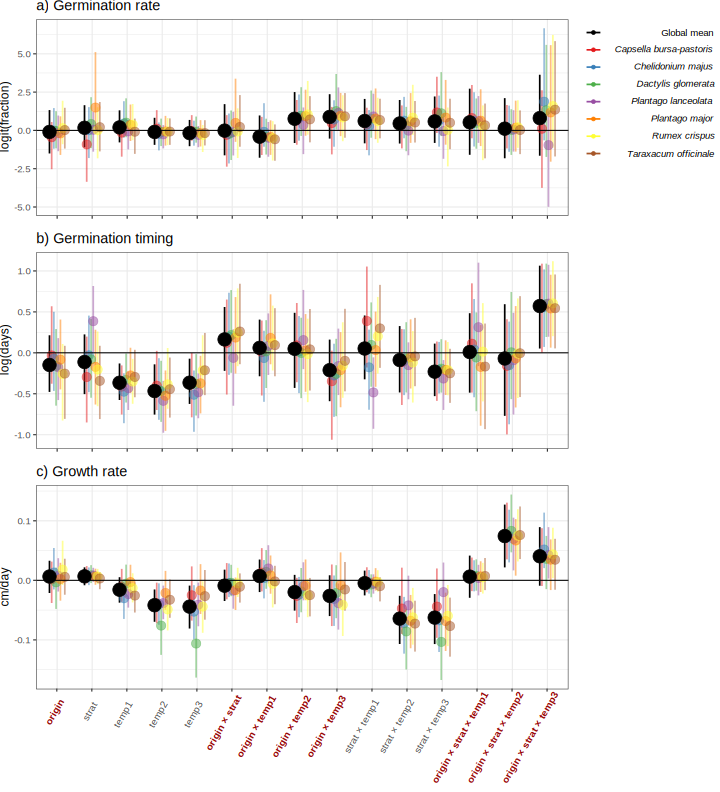
\includegraphics[scale=.5,angle=-90]{germ_figs_onepage.pdf}}
	\caption{Hierarchical mixed-effects model coefficients with 95\% credibility intervals, showing global average effects and species random effects. a) model of germination rate (plogit(\% germination)). b) model of germination day (log(day)) and c) model of growth rate (cm/day)}
	\label{fig:coef}
\end{figure}
	
%	\includepdf[pages={2,1,3},width=\textwidth]{germ_figs.pdf}
%	\begin{figure}
%		\fbox{\includegraphics[page=2,scale=.8]{germ_figs.pdf}}
%			\caption{Germination rate model coefficients}
%			\label{fig:ratecoef}
%	\end{figure}
%\begin{figure}
%	\fbox{\includegraphics[page=1,scale=.8]{germ_figs.pdf}}
%	\caption{Germination day model coefficients}
%	\label{fig:timecoef}
%\end{figure}
%
%\begin{figure}
%	\fbox{\includegraphics[page=3,scale=.8]{germ_figs.pdf}}
%	\caption{Growth rate model coefficients}
%	\label{fig:grcoef}
%\end{figure}
%	
%	\begin{sidewaysfigure}[h!]
%		\begin{subfigure}[b]{.5 \textheight}
%			\caption{}
%			\includegraphics[page=2,scale=.5,width=\textwidth]{germ_figs.pdf}
%		\end{subfigure}
%	\begin{subfigure}[b]{.5 \textheight}
%			\caption{}
%			\includegraphics[page=1,width=\textwidth]{germ_figs.pdf}
%		\end{subfigure}
%	\begin{subfigure}[b]{.5 \textheight}
%			\caption{}
%			\includegraphics[page=3,width=\textwidth]{germ_figs.pdf}
%		\end{subfigure}
%		\caption{Blah.}
%	\end{sidewaysfigure}
		
		%,scale=.5,angle=90]{germ_figs.pdf}
	%			\includegraphics[page=1,scale=.5,angle=90]{germ_figs.pdf}
%				\includegraphics[page=3,scale=.5,angle=90]{germ_figs.pdf}}
	%	%x x x lower right 
	%	\caption{Model coefficients}
	%	\label{fig:coef}
	%\end{figure}		
	\section{Discussion} 
	
	My study investigated key mechanisms that enable plants to invade new environments. My experiments tested for phenological local adaptation and plasticity across seven herbaceous species. We found no general patterns in adapted plasticity across phenologies or species.  However, We did find that invasive populations consistently showed evidence of local adaptation to the alien environment for germination timing and growth rate. Yet, sign of a local adaptation for germination rate was limited to two species.  Generally, my results show that invasive plants are able to adapt to novel climates, suggesting that they will become only more invasive in the face of global climate change. 
	
	\subsection{Germination Rate} 
	
	
	Germination rate (i.e., the percent of seeds that successfully germinated) did not differ between population origins and across growing conditions for most species. For all species except Plantago major and Capsella bursa-pastoris, germination rate was not significantly affected by temperature, stratification length, or population origin. This suggests that germination rate is generally not sensitive to temperature or stratification length. Further, it suggests that, generally, the US and European populations have not diverged with regards to germination rate. 
	
	The lack of difference in germination rates between the European and US suggests that germination rate has not evolved post-introduction. Consequently, the contribution of germination rate adaptability to invasive success is likely quite small. 
	
	Germination rate in two species, however, differed between the population origins. Germination rates of Plantago major and Capsella bursa-pastoris were dependent on population origin, while that of Plantago major was also dependent on stratification length. Stratification is an important determinant of germination rate, at least for the US Plantago major. This suggests that at least two invasive species have diverged from their native origins with respect to germination rate. 
	
	This divergence of germination rate in the US may be a result of adaptation to local environments.  The invasive US members of Plantago major and Capsella bursa-pastoris have equal or lower germination rates than their European conspecifics. So how does this adaptation for low germination rate possibly confer a fitness benefit? Perhaps there were stratification and temperature combinations that we did not measure at which the US would have performed much better (i.e. these species have adapted to very specific local conditions, which were not contained within our treatment conditions). Local adaptation may be important in giving these Plantago major and Capsella bursa-pastoris the ability to thrive in novel environments.
	
	Local adaptation, however, is not the only explanation for these observed differences between US and European populations. A higher germination rate may not in fact be beneficial to fitness—perhaps some seeds germinated at low rates because they have a long seedbank life and have adapted to only germinate under ideal conditions. Or perhaps the differences could be a result of nonadaptive genetic drift, aided by the initially small introduced population size. The differences could also be caused by the founder effect—e.g., the genotypes that happened to be introduced to the US already had the observed differentiated genotype, and hence all of their progeny did as well. However, an extensive diversity of native populations were sampled and local adaptation is known to have occurred in some invasive species (e.g., Lamarque et al., 2014). Thus, while acknowledging that there may be alternate explanations for the observed phenology differences, we will focus my discussion on local adaptation where appropriate.  
	
	Local adaptation may be important for the US population origins of these two species, but US populations actually display less plasticity. The US \textit{Capsella bursa-pastoris} and \textit{Plantago major} showed higher individual-level variation in germination rates than the European populations, while all the other species showed no significant difference between origins. This suggests that for germination rate, the US populations of some species are locally adapted and less plastic. This inverse relationship between plasticity and local adaptation of the invasive population makes sense. If these species have adapted to germinate well only in specific conditions, then it should follow that germination is less plastic. 
	
	
	\subsection{Germination Timing}
	
	
	Unlike germination rate, germination timing was significantly different across population origins and growing conditions for all species except Capsella bursa-pastoris. Germination timing for all of these species was significantly affected by each of temperature, stratification length, and population origin. This suggests that, unlike germination rate, germination timing is generally sensitive to temperature and stratification length. Further, the significance of origin effects suggests that the US and Europe have diverged with respect to germination timing. 
	
	Adaptation of germination timing may be a driver of invasion success for most species. The significant differences in germination timing between the European and US suggest that germination timing has possibly evolved since introduction of the invaders.  
	
	These adaptations could be proof that some species can adapt their phenologies. For example, in nearly all of the species in the shorter stratification, the US germination time was significantly different from that of Europe. This suggests that the US plants have evolved to respond differently to the shorter stratification—i.e., a shorter winter—than the European plants. These local adaptations display the ability of these plants to adapt their germination timing to altered winter lengths. 
	
	Further, this phenological adaptability could yield an invasive advantage. For example, in the shorter stratification, Chelidonium majus germinated significantly earlier in the US than in Europe. This flexibility to the short stratification could mean that the US Chelidonium majus is germinating earlier to taking advantage of a vacant niche or wealth of resources in the early spring. This ability to take advantage of resources could make it a more successful invader. 
	
	These adaptations may not only benefit invaders in a stable climate, but may also render some species more invasive in a changing climate.  For example, since cold-stratification is a simulation of temperate winter, the evidence that species can adapt their germination timing in accordance with a shorter stratification length, suggests that they may be well positioned to germinate in a climate with shorter winters. Winters are forecasted to get shorter due to climate change (IPCC, 2015), thus these already invasive species may become even more invasive as the climate changes. 
	
	There is no general result on the importance of plasticity in germination timing. Some species showed significantly higher variation in the US origin than the European origin, some showed lower, and some exhibited no significant difference. For example, the US origin of Chelidonium majus showed more variability in germination timing than the European origin, while Taraxacum officinale displayed the opposite. This implies that the US Taraxacum officinale may have greater plasticity those from Europe.  However, plasticity per se does not necessarily give a plant an invasive advantage. To impart invasiveness, the plastic trait must be a fitness trait (Richards et al., 2006). Generally, higher germination rates impart higher fitness. However fitness is not necessarily correlated with timing of germination. There may be some environments in which germinating earlier could be beneficial (e.g., there’s a short growing season or presence of upper-story trees that will shade understory plants) whereas other times germinating later may be beneficial (e.g., less risk from frost damage). Thus while plasticity has increased for some species in the US, it may not have directly increased their invasion potential. More work is needed to analyze how germination timing interacts with fitness for these species before germination timing variability and invasiveness can be clearly connected.  
	
	\subsection{Growth Rate}
	
	Like germination timing, growth rate was significantly different across population origins and growing conditions for nearly all species. Growth rate was significantly affected by temperature, stratification length, and population origin for all species except Dactylis glomerata (which was only affected by temperature). This suggests that, like germination timing, growth rate is generally sensitive to temperature and stratification length. 
	
	Growth rate is controlled by the interaction of stratification length and temperature. In general, growth rate decreased as temperature increased for all species. This could cause plants to grow more slowly as the planet warms due to anthropogenic forcing of the climate system. However, the decrease in growth rate was generally less severe for the shorter stratification. This suggests that warming temperatures will have a less dramatic effect on growth rate if they are accompanied by shorter winters. Understanding how plants will react to climate change requires taking both winter and summer climate effects into account. 
	
	
	Growth rate is also significantly dependent on population origin for all species (except Dactylis glomerata), suggesting that the US and European growth rate have diverged. In nearly all of the species the effect of temperature and/or stratification varied by population origin. The US has evolved to respond differently to stratification and/or temperature. These local adaptations display the flexibility of growth rate to stratification length and temperature. 
	
	This phenological adaptability could yield an invasive advantage. For example, the US Plantago lanceolata grew significantly faster than those from Europe at mid-temperatures, but equal to or slower than at extreme temperatures. This adaptability to temperature could mean that the US Plantago lanceolata has locally adapted to grow faster at mid-range temperatures in our study. This could allow US populations to take advantage of a vacant niche for taller plants or wealth of resources only available to taller plants in and mid-temperature abiotic environment. This ability to take advantage of resources could make it a more successful invader. Additionally, these adaptations may make some species more invasive in a changing climate. For example, the evidence that the relationship between growth rate and temperature is flexible suggests that these species may be able to adapt their growth rate to changing temperatures. Thus these species may become even more invasive as the climate changes.
	
	As with plasticity of germination timing, we found no general answer on whether plasticity has increased in the US populations. Some species showed significantly higher normalized variation in the US than in Europe, some showed lower, and one exhibited no significant difference. For example, the US and European Plantago lanceolata showed no difference, whereas the US Chelidonium majus was significantly less variable than that from Europe. This suggests that the US Chelidonium majus has adapted to have a more plastic growth rate. However, as with germination timing, using trait plasticity to imply invasiveness is tricky if the trait is not clearly a fitness trait.  Nevertheless, a higher growth rate should typically yield a greater fitness, and so plasticity may play an important role in imparting invasiveness in US Chelidonium majus, Dactylis glomerata, Rumex crispus, and Taraxacum officinale.  
	
	
	\section{Conclusion}
	
	
	Germination rate is not dependent on stratification or temperature for most species, and most species are similar in both the native and invasive origins for this trait. However, some species show signs of local adaptation, and lower derived plasticity in the invasive origin. 
	
	Germination timing and growth rate are sensitive to stratification length and temperature for nearly all species. Plants in the US have adapted to respond to these environmental conditions significantly differently than those from Europe. The US populations in some species have also evolved greater or lesser variability relative to the European population, suggesting that they may have evolved more or less plasticity. Thus, while plasticity may be important for some species but not for others, local adaptation seems to be a common strategy among herbaceous plant invaders. 
	
	These adaptations have likely contributed to the US plants becoming better invaders. They have perhaps allowed these plants to thrive in their novel introduction sites. In demonstrating their ability to adapt to local environments, these plants have shown that they may be able to excel in diverse climates. Their capacity to adapt to different winter lengths and temperatures in the US will also allow them to adapt to the novel seasons and temperatures associated with global climate change.  
	
	In the future, invasive plants may become increasingly significant elements of our changing planet’s ecosystems. As such, future research is needed to further elucidate the mechanisms by which plants become invasive and thrive in a changing climate. 
	
	
	\section{Acknowledgments}
	 The field work for this thesis was generously funded by the Harvard College Research Fund and the Harvard University Center for the Environment Undergraduate Summer Research Fund. Thanks to Beth Forrestel for mentorship to HNE. Thanks also to Dan Flynn, Sally Gee, Jehane Samaha, and Tim Savas for help transplanting, sampling, and data collection. Thanks to Faye Rosin, Kea Woodruff, and Jess Gard for help with collection and growing logistics. Thanks to S. Fritz for help with data input. Thank you to M. Rucinski, C. Husic, N. Gilbert, A. Delgado, and A. Acosta for comments on earlier versions of this paper. Thanks to J. Eyster, S. Stalhandske, and G. Barbone for assistence with and camaraderie during field sampling. 

	

\section{Literature Cited}
%\printbibliography
\end{document}
